\documentclass{article}
\usepackage{graphicx}

\usepackage[spanish]{babel}
\usepackage[utf8]{inputenc}
\usepackage[T1]{fontenc}

\usepackage[margin=1in]{geometry}
\usepackage{graphicx}
\usepackage{booktabs}
\usepackage{amsmath, amssymb}
\usepackage{siunitx}            
\usepackage{caption}
\usepackage{subcaption}
\usepackage{hyperref}
\usepackage{enumitem}
\usepackage{float}             
\usepackage{xcolor}
\usepackage{adjustbox}
\usepackage{graphicx}   


\usepackage[backend=biber,style=apa]{biblatex}

\addto\captionsspanish{%
  \renewcommand{\tablename}{Tabla}%
  \renewcommand{\listtablename}{Índice de tablas}%
}


\title{Algoritmos supervisados y no supervisados aplicados a analizar la relación entre la salud mental, hábitos y felicidad.}
\author{Fisam Zavala | Maestría en Ciencia de Datos | Aprendizaje Automático}
\date{Noviembre 2025}

\begin{document}
\maketitle


                    \section{Introducción}

El bienestar y la salud mental se han convertido en temas centrales de investigación en las ciencias sociales y del comportamiento, especialmente ante el aumento de factores que afectan la calidad de vida en entornos modernos. Los avances recientes en el aprendizaje automático han permitido analizar estas variables desde un enfoque cuantitativo, facilitando la identificación de patrones y relaciones complejas entre los hábitos de vida, las emociones y la percepción de felicidad.

En este contexto, el presente estudio busca analizar cómo distintos factores del estilo de vida —tales como el sueño, el nivel de estrés, el tipo de dieta, las horas de trabajo y la interacción social— se relacionan con los niveles de bienestar subjetivo y felicidad. Para ello, se aplicaron algoritmos de aprendizaje supervisado y no supervisado con el objetivo de explorar tanto la estructura interna de los datos como su capacidad predictiva.

El enfoque metodológico combina técnicas de agrupamiento, como \textit{K-Means} y \textit{DBSCAN}, con modelos de predicción basados en regresión lineal y selección de características (\textit{SelectKBest} y \textit{RFE}), además de estrategias para evaluar el número óptimo de clústeres y los errores de estimación. Esta integración de métodos permite abordar el análisis desde una perspectiva exploratoria y explicativa, contribuyendo a una mejor comprensión de los determinantes del bienestar.

En suma, el propósito de este trabajo es identificar patrones de bienestar y evaluar la influencia de los hábitos personales sobre la salud mental y la felicidad percibida, demostrando cómo el aprendizaje automático puede constituirse en una herramienta eficaz para el análisis interdisciplinario del comportamiento humano.


                    \section{Descripción de los datos}


En la Tabla~\ref{tab:ed1} se presenta la estadística descriptiva univariada de las variables numéricas del estudio. En términos generales, se observa que las horas de sueño presentan una media de 6.48 horas, con baja dispersión (desviación estándar de 1.50), lo cual sugiere que la mayoría de los individuos mantiene rutinas de descanso relativamente constantes. Por otro lado, las horas trabajadas por semana muestran una variabilidad considerable (varianza de 131.14 y desviación estándar de 11.45), evidenciando diferencias significativas en las cargas laborales entre los participantes.

\begin{table}[H]
\centering
\resizebox{\textwidth}{!}{%
  \begin{tabular}{lrrrrrrr}
\toprule
 & Media & Mediana & Moda & Varianza & Desv. estándar & Q1 & Q3 \\
\midrule
Sleep Hours & 6.480000 & 6.500000 & 6.600000 & 2.250000 & 1.500000 & 5.500000 & 7.500000 \\
Work Hours per Week & 39.470000 & 39.000000 & 26.000000 & 131.140000 & 11.450000 & 30.000000 & 50.000000 \\
Screen Time per Day (Hours) & 5.090000 & 5.100000 & 6.700000 & 3.050000 & 1.750000 & 3.600000 & 6.600000 \\
Social Interaction Score & 5.470000 & 5.500000 & 4.500000 & 6.570000 & 2.560000 & 3.300000 & 7.600000 \\
Happiness Score & 5.400000 & 5.400000 & 2.900000 & 6.540000 & 2.560000 & 3.200000 & 7.500000 \\
\bottomrule
\end{tabular}
 
}
\caption{Estadística Descriptiva.}
\label{tab:ed1}
\end{table}

La Figura~\ref{fig:ed2} muestra la distribución de estas variables, donde se aprecia que ninguna presenta forma claramente normal: el sueño tiende a ser unimodal y ligeramente sesgado a la derecha, mientras que las horas de uso de pantalla y el puntaje de felicidad muestran una distribución más uniforme, lo que sugiere heterogeneidad en los hábitos tecnológicos y en el bienestar emocional.

\begin{figure}[H]
    \centering
    \includegraphics[width=0.8\textwidth]{figures/est_descriptiva_histogramas.png}
    \caption{}
    \label{fig:ed2}
\end{figure}

En relación con los niveles de dispersión, la Figura~\ref{fig:ed3} evidencia que las horas trabajadas por semana concentran el mayor rango intercuartílico, lo cual coincide con la alta variabilidad reportada en la Tabla~\ref{tab:ed1}. En contraste, variables como interacción social y uso de pantallas presentan rangos intercuartílicos más reducidos, indicando comportamientos más homogéneos entre los sujetos del estudio.

\begin{figure}[H]
    \centering
    \includegraphics[width=0.7\textwidth]{figures/est_descriptiva_rango.png}
    \caption{}
    \label{fig:ed3}
\end{figure}

Finalmente, los diagramas de correlación de Pearson y Spearman (Figuras~\ref{fig:ed4} y ~\ref{fig:ed44}) muestran que no existe una relación lineal o monotónica fuerte entre las variables cuantitativas. En particular, la relación entre horas de sueño, interacción social y horas de trabajo tiende a ser cercana a cero, lo cual sugiere que estas variables pueden requerir técnicas de análisis no lineales o modelos que capturen relaciones más complejas. Según estas observaciones iniciales, no se esperarían problemas de multicolinealidad en los modelos posteriores de predicción.

\begin{figure}[H]
    \centering
    \includegraphics[width=0.7\textwidth]{figures/pearsoncorr.png}
    \caption{}
    \label{fig:ed4}
\end{figure}

\begin{figure}[H]
    \centering
    \includegraphics[width=0.6\textwidth]{figures/spearmancorr.png}
    \caption{}
    \label{fig:ed44}
\end{figure}


                    \section{Antecedentes}

Diversos estudios han abordado la relación entre los hábitos de vida, la salud mental y la felicidad, empleando enfoques cuantitativos y técnicas de aprendizaje automático para identificar patrones de bienestar. 

En el estudio realizado por el \textit{Journal of Pakistan Medical Students} (JPMS, 2021), se exploró cómo los hábitos de vida auto–reportados, tales como las horas de sueño, el tiempo frente a pantalla y los niveles de estrés, pueden predecir el grado de felicidad mediante modelos de minería de datos y aprendizaje automático. Los resultados mostraron que la calidad del sueño y la gestión del estrés son variables determinantes en los niveles de bienestar subjetivo.

Por su parte, la investigación publicada en \textit{BMC Public Health} (2019) destacó una relación longitudinal entre el optimismo, la felicidad y los comportamientos saludables, demostrando que el bienestar emocional no solo depende de los hábitos, sino que también puede influir en su mantenimiento a lo largo del tiempo. 

De manera complementaria, el artículo de \textit{Preventive Medicine Reports} (2021) evidenció que el bienestar subjetivo predice conductas de salud a largo plazo, reforzando la hipótesis de una relación bidireccional entre bienestar psicológico y estilo de vida saludable. 

Más recientemente, el estudio publicado en \textit{Scientific Reports} (Nature Portfolio, 2025) empleó modelos gráficos para analizar la interacción entre múltiples dimensiones del bienestar, incluyendo el sueño, las relaciones sociales y la satisfacción laboral. Dicho trabajo concluye que los factores emocionales y sociales se encuentran estrechamente interconectados en la percepción global de bienestar.

Finalmente, el artículo del \textit{International Journal of Qualitative Studies on Health and Well-Being} (2023) analizó la influencia de la alimentación en la percepción de bienestar infantil, encontrando que los hábitos alimenticios diarios están vinculados con la estabilidad emocional y la satisfacción personal.

En conjunto, estos antecedentes muestran que la felicidad y la salud mental están fuertemente asociadas con los hábitos de vida, y que las metodologías basadas en aprendizaje automático ofrecen un marco eficaz para modelar y comprender dichas relaciones complejas.

                    \section{Marco Teórico}

\subsection{Métricas de desempeño}

La evaluación del desempeño de los modelos predictivos es esencial para determinar su capacidad de generalización y precisión. En el caso de los modelos de regresión, las métricas se centran en medir el error entre los valores observados y los valores predichos. A continuación, se describen las principales métricas utilizadas en este trabajo: el Error Absoluto Medio (MAE), el Error Cuadrático Medio (MSE), la Raíz del Error Cuadrático Medio (RMSE) y el Coeficiente de Determinación ($R^2$).

\subsubsection{Error Absoluto Medio (MAE)}

El \textit{Mean Absolute Error} (MAE) mide el promedio de las diferencias absolutas entre los valores reales ($y_i$) y los valores predichos ($\hat{y_i}$). Su fórmula se expresa como:

\begin{equation}
    MAE = \frac{1}{n} \sum_{i=1}^{n} | y_i - \hat{y_i} |
\end{equation}

El MAE representa la magnitud promedio del error de predicción, expresado en las mismas unidades que la variable objetivo. Es una métrica robusta ante valores atípicos y fácil de interpretar, ya que indica, en promedio, cuánto se desvía el modelo de los valores reales.

\subsubsection{Error Cuadrático Medio (MSE)}

El \textit{Mean Squared Error} (MSE) calcula el promedio de los errores al cuadrado entre los valores observados y los estimados. Se define como:

\begin{equation}
    MSE = \frac{1}{n} \sum_{i=1}^{n} ( y_i - \hat{y_i} )^2
\end{equation}

El MSE penaliza con mayor peso los errores grandes debido a la elevación al cuadrado, por lo que resulta útil cuando se desea dar más importancia a desviaciones significativas. No obstante, su interpretación directa puede ser menos intuitiva al no estar en las mismas unidades de la variable dependiente.

\subsubsection{Raíz del Error Cuadrático Medio (RMSE)}

La \textit{Root Mean Squared Error} (RMSE) es la raíz cuadrada del MSE, y se calcula como:

\begin{equation}
    RMSE = \sqrt{\frac{1}{n} \sum_{i=1}^{n} ( y_i - \hat{y_i} )^2}
\end{equation}

El RMSE conserva las unidades originales de la variable objetivo, lo que facilita su interpretación. Es sensible a los valores atípicos, pero proporciona una visión clara del error promedio esperado en las predicciones. En comparación con el MAE, el RMSE tiende a ser mayor cuando existen errores extremos.

\subsubsection{Coeficiente de Determinación ($R^2$)}

El \textit{Coeficiente de Determinación}, denotado como $R^2$, mide la proporción de la variabilidad total de los datos que es explicada por el modelo. Su expresión matemática es:

\begin{equation}
    R^2 = 1 - \frac{SS_{res}}{SS_{tot}} = 1 - \frac{\sum_{i=1}^{n} (y_i - \hat{y_i})^2}{\sum_{i=1}^{n} (y_i - \bar{y})^2}
\end{equation}

Donde $SS_{res}$ es la suma de los residuos al cuadrado y $SS_{tot}$ representa la variabilidad total de los datos respecto a su media. El valor de $R^2$ varía entre 0 y 1, siendo los valores cercanos a 1 indicativos de un buen ajuste del modelo. Sin embargo, un $R^2$ elevado no garantiza que el modelo sea el más adecuado, por lo que debe interpretarse junto con las métricas de error.



\subsection{Diseño de Experimentos}
\label{subsec:doe}

\subsubsection{Selección de factores y niveles}
\label{subsubsec:factores}
Se consideran factores centrales por plausibilidad causal y disponibilidad en el dataset. Para variables continuas, se dicotomizan en niveles \emph{bajo/alto} usando la mediana muestral; esto balancea tamaños de grupo y simplifica un diseño $2^k$.

\begin{table}[H]
\centering
\caption{Factores y niveles propuestos (umbrales según mediana muestral).}
\label{tab:factores_niveles}
\begin{tabular}{llp{7.5cm}}
\toprule
\textbf{Factor} & \textbf{Niveles} & \textbf{Definición operacional} \\
\midrule
Exercise Level & Bajo / Alto & Según codificación del dataset (p.ej., Low vs High). \\
Sleep Hours & Bajo / Alto & $\leq 6.5$ h vs $> 6.5$ h. \\
Stress Level & Bajo / Alto & Low vs High (excluir \emph{Moderate} o recodificar a binario). \\
Diet Type & Balanceada / No balanceada & Balanced vs (Vegan/Vegetarian/Junk Food) o criterio nutricional equivalente. \\
Work Hours per Week & Bajo / Alto & $\leq 39$ h/sem vs $> 39$ h/sem. \\
Screen Time per Day (Hours) & Bajo / Alto & $\leq 5.1$ h/día vs $> 5.1$ h/día. \\
Social Interaction Score & Bajo / Alto & $\leq 5.5$ vs $> 5.5$. \\
\bottomrule
\end{tabular}
\end{table}

\subsubsection{Estructura del diseño}
\label{subsubsec:estructura}
Incluir los siete factores anteriores en un factorial completo implicaría $2^7 = 128$ tratamientos. Para controlar el tamaño del experimento sin perder capacidad de \emph{screening}, se propone un \textbf{diseño fraccional factorial} de resolución IV:
\[
2^{7-3} = 16 \text{ tratamientos (Resolución IV),}
\]
el cual permite estimar \emph{efectos principales} libres de confusión con interacciones de dos factores (aunque las interacciones dobles pueden estar aliadas entre sí). Alternativamente, si se desea más poder para interacciones, puede considerarse $2^{7-2} = 32$ corridas.

\paragraph{Fase 1 (screening).} Aplicar el $2^{7-3}$ (o $2^{7-2}$) con aleatorización y, de ser posible, 1–2 réplicas técnicas para estimar error puro. Analizar con ANOVA factorial (modelo lineal con efectos principales y, opcionalmente, interacciones seleccionadas).

\paragraph{Fase 2 (optimización).} Con los 2–3 factores más influyentes, pasar a una \textbf{Superficie de Respuesta} (p.ej., Diseño Central Compuesto) para capturar curvatura y encontrar combinaciones que maximizan \textit{Happiness Score}.

\subsubsection{Modelo y análisis}
\label{subsubsec:analisis}
Sea $Y$ el \textit{Happiness Score} y $X_j$ los indicadores (0/1) de los niveles altos de cada factor. El modelo lineal para la fase de \emph{screening} es:
\[
Y \;=\; \beta_0 + \sum_{j=1}^{k} \beta_j X_j \;+\; \sum_{j<\ell} \beta_{j\ell} X_j X_\ell \;+\; \varepsilon, 
\quad \varepsilon \sim \mathcal{N}(0,\sigma^2).
\]
Se contrasta significancia de efectos principales e interacciones mediante ANOVA y pruebas $F$, verificando supuestos (normalidad de residuos, homocedasticidad e independencia). Para el dataset observacional actual, el mismo marco puede implementarse como \textbf{AN(C)OVA}, añadiendo covariables (p.ej., Age, Country) o usando \emph{blocking} conceptual.


                    \section{Metodología}

\subsection{Selección de características}

En el aprendizaje supervisado, la selección de características constituye una etapa fundamental para reducir la dimensionalidad del conjunto de datos, mejorar la interpretabilidad del modelo y evitar el sobreajuste (\textit{overfitting}). En este estudio se emplearon tres enfoques distintos: \textit{SelectKBest – F (f\_regression)}, \textit{SelectKBest – Mutual Information (MI)} y \textit{Recursive Feature Elimination (RFE)} con \textit{LinearRegression}. Cada uno aborda la relevancia de las variables desde una perspectiva distinta: estadística, informacional y de desempeño predictivo, respectivamente.

\subsubsection{SelectKBest – F (f\_regression)}

Este método utiliza la prueba F derivada del análisis de varianza (ANOVA) para evaluar la relación lineal entre cada variable independiente $X_i$ y la variable objetivo $y$.  
El estadístico F se define como:

\[
F = \frac{MS_{\text{entre}}}{MS_{\text{dentro}}} = \frac{\text{Varianza explicada por el modelo}}{\text{Varianza residual}}
\]

donde $MS_{\text{entre}}$ representa la variabilidad media entre los grupos definidos por $X_i$ y $MS_{\text{dentro}}$ la variabilidad interna o error.  
Un valor alto de $F$ indica que la variable $X_i$ tiene una influencia significativa sobre $y$, lo que sugiere que debe ser considerada en el modelo.

\subsubsection{SelectKBest – Mutual Information (MI)}

El método basado en información mutua cuantifica la dependencia estadística (no necesariamente lineal) entre dos variables aleatorias.  
La \textit{Mutual Information} (MI) mide cuánta información de $X_i$ reduce la incertidumbre de $y$ y se define como:

\[
I(X;Y) = \sum_{x \in X} \sum_{y \in Y} p(x,y) \log\left( \frac{p(x,y)}{p(x)p(y)} \right)
\]

donde $p(x,y)$ es la distribución conjunta y $p(x)p(y)$ el producto de las marginales.  
A diferencia de la prueba F, la MI detecta dependencias tanto lineales como no lineales, siendo especialmente útil cuando la relación entre las variables no sigue un patrón paramétrico.

\subsubsection{Recursive Feature Elimination (RFE) con LinearRegression}

El método RFE selecciona características de forma iterativa eliminando las menos relevantes en función del peso que aportan al modelo.  
Se entrena una regresión lineal sobre todas las variables y se calculan los coeficientes $\beta_i$ asociados a cada predictor $X_i$.  
En cada iteración se eliminan las variables con menor valor absoluto de $\beta_i$, repitiendo el proceso hasta conservar el número óptimo de características $k$.

El modelo lineal de base se define como:

\[
\hat{y} = \beta_0 + \sum_{i=1}^{p} \beta_i X_i
\]

donde $\beta_i$ indica la contribución de la variable $X_i$ sobre la variable dependiente $\hat{y}$.  
De esta forma, RFE busca identificar el subconjunto de variables que maximiza el desempeño predictivo del modelo lineal minimizando simultáneamente el error cuadrático medio (MSE).

\subsection{Algoritmos no supervisados}

Los algoritmos no supervisados permiten descubrir estructuras o patrones ocultos en los datos sin requerir una variable objetivo. En este trabajo se aplicaron dos técnicas de agrupamiento: \textit{K-Means} y \textit{DBSCAN}, complementadas con diversos criterios para determinar el número óptimo de clústeres. Estos métodos permiten segmentar observaciones con base en su similitud multivariada, identificando grupos representativos del comportamiento general de la población analizada.

\subsubsection{K-Means Clustering}

El algoritmo \textit{K-Means} busca dividir el conjunto de datos en $k$ grupos homogéneos de tal forma que se minimice la distancia interna entre las observaciones y el centroide de su respectivo clúster.  
Matemáticamente, su objetivo consiste en minimizar la suma total de las distancias cuadráticas intra–clúster:

\[
J = \sum_{i=1}^{k} \sum_{x_j \in C_i} \| x_j - \mu_i \|^2
\]

donde $C_i$ representa el conjunto de observaciones asignadas al clúster $i$, y $\mu_i$ es el centroide correspondiente, definido como el promedio de las observaciones de dicho grupo.  
El algoritmo sigue un proceso iterativo de dos pasos: (1) asignación de puntos al centroide más cercano y (2) actualización de los centroides hasta alcanzar convergencia o un cambio mínimo en $J$.

\subsubsection{DBSCAN (Density-Based Spatial Clustering of Applications with Noise)}

A diferencia de K-Means, el algoritmo \textit{DBSCAN} agrupa observaciones con base en la densidad de puntos en el espacio de características, lo que le permite identificar clústeres de forma arbitraria y detectar valores atípicos (\textit{outliers}).  
Cada punto se clasifica como núcleo, frontera o ruido según dos parámetros: la distancia máxima $\varepsilon$ y el número mínimo de puntos requeridos \textit{MinPts}.

Formalmente, un punto $p$ es considerado núcleo si cumple que:

\[
|\{ q \in D \mid \text{dist}(p,q) \leq \varepsilon \}| \geq \text{MinPts}
\]

Los clústeres se forman a partir de la conectividad entre puntos núcleo y sus vecinos directos, mientras que los puntos no alcanzables por densidad se consideran ruido.  
Este enfoque es especialmente útil para conjuntos de datos con distribuciones irregulares o presencia significativa de anomalías.

\subsubsection{Estrategias para determinar el número óptimo de clústeres}

La determinación del número adecuado de clústeres ($k$) es un aspecto crítico en los algoritmos de agrupamiento. Para ello, se aplicaron tres estrategias complementarias: el \textit{Método del Codo}, el \textit{Coeficiente de Silhouette} y el \textit{Índice de Calinski–Harabasz}.

\paragraph{Método del Codo}

Evalúa la función de costo $J(k)$ definida como la suma de las distancias intra–clúster para diferentes valores de $k$.  
El número óptimo de clústeres se elige donde la reducción marginal de $J(k)$ comienza a estabilizarse, formando un “codo” en la gráfica:

\[
J(k) = \sum_{i=1}^{k} \sum_{x_j \in C_i} \| x_j - \mu_i \|^2
\]

\paragraph{Coeficiente de Silhouette}

Mide la cohesión y separación de los clústeres mediante la comparación entre la distancia promedio de un punto a los elementos de su propio grupo ($a_i$) y la distancia promedio al clúster más cercano ($b_i$):

\[
s_i = \frac{b_i - a_i}{\max(a_i, b_i)}
\]

El valor promedio de $s_i$ para todos los puntos varía entre $-1$ y $1$, donde valores cercanos a $1$ indican clústeres bien definidos.

\paragraph{Índice de Calinski–Harabasz}

También conocido como el \textit{Variance Ratio Criterion}, este índice evalúa la proporción entre la dispersión inter–clúster y la dispersión intra–clúster:

\[
CH = \frac{\text{Tr}(B_k) / (k - 1)}{\text{Tr}(W_k) / (n - k)}
\]

donde $\text{Tr}(B_k)$ es la traza de la matriz de dispersión entre clústeres y $\text{Tr}(W_k)$ la traza de la matriz de dispersión interna.  
Un valor más alto de $CH$ indica una mejor partición de los datos.


\subsection{Algoritmos Supervisados}

Los algoritmos supervisados utilizan un conjunto de datos etiquetados, donde las variables predictoras $X$ se asocian con una variable respuesta $y$. El objetivo es construir una función $f(X)$ capaz de aproximar el valor de $y$ para nuevas observaciones, minimizando el error entre los valores observados y los predichos.

$$
y_i = f(X_i) + \varepsilon_i, \quad \text{con } \varepsilon_i \sim N(0, \sigma^2)
$$

A continuación se describen algunos de los algoritmos supervisados más comunes utilizados en problemas de regresión y pronóstico:

\subsubsection{Regresión Lineal}

Busca establecer una relación lineal entre la variable dependiente y las variables independientes. Su formulación matemática general es:
$$
\hat{y}*i = \beta_0 + \beta_1 x*{i1} + \beta_2 x_{i2} + \dots + \beta_p x_{ip}
$$
Los coeficientes $\beta_j$ se estiman minimizando la suma de los errores cuadráticos:
$$
\min_{\beta} \sum_{i=1}^{n} (y_i - \hat{y}*i)^2 = \min*{\beta} (y - X\beta)'(y - X\beta)
$$
La solución analítica se obtiene mediante:
$$
\hat{\beta} = (X'X)^{-1}X'y
$$
Es un modelo interpretable y constituye la base para la mayoría de los métodos de regresión.

\subsubsection{Regresión de Bosques Aleatorios (Random Forest)}

Es un método de ensamble basado en múltiples árboles de decisión. Cada árbol $T_b$ se entrena sobre una muestra aleatoria $S_b$ del conjunto original. La predicción final se obtiene promediando las salidas de todos los árboles:
$$
\hat{y} = \frac{1}{B} \sum_{b=1}^{B} T_b(X)
$$
donde $B$ representa el número de árboles en el bosque. Este método reduce la varianza del modelo y mejora la generalización.



                    \section{Resultados}


Una etapa fundamental en el uso de \textit{K-Means} es definir el número adecuado de clústeres (\(k\)), ya que este parámetro influye directamente en la estructura final del agrupamiento.  
Existen diversas métricas de validación interna que permiten evaluar la calidad de las particiones obtenidas. En este análisis se emplearon dos de las más utilizadas:

\begin{itemize}
    \item \textbf{Método del Codo (Elbow Method):} evalúa la \textit{inercia}, es decir, la suma de las distancias cuadráticas entre los puntos y su centroide correspondiente. Se calcula para distintos valores de \(k\), y el valor óptimo se identifica en el punto donde la disminución de la inercia deja de ser significativa, formando un “codo” en la gráfica.

    \item \textbf{Coeficiente de Silhouette:} mide la calidad de la asignación de cada observación a su clúster, comparando la distancia promedio al resto de los puntos del mismo grupo con la distancia promedio al clúster más cercano. Valores cercanos a 1 indican una buena separación entre clústeres, mientras que valores negativos sugieren una posible asignación errónea.
\end{itemize}

Ambos métodos se aplicaron para el rango \(k = 2 \text{ a } 10\), encontrándose que el punto de inflexión en el método del codo y el máximo promedio del coeficiente de Silhouette coincidieron aproximadamente en \(k = 3\), lo cual sirvió como guía para la selección inicial del número de grupos.  

\begin{figure}[H]
    \centering
    \includegraphics[width=0.6\textwidth]{figures/elbow.png}
    \caption{Método del Codo: se observa una disminución pronunciada en la inercia hasta \(k=3\), 
    punto a partir del cual la reducción se estabiliza, sugiriendo que tres clústeres son apropiados.}
    \label{fig:elbow_method}
\end{figure}

\begin{figure}[H]
    \centering
    \includegraphics[width=0.6\textwidth]{figures/silhouette.png}
    \caption{Coeficiente de Silhouette por número de clústeres. Los valores más altos 
    indican una mejor cohesión dentro de los grupos y una mayor separación entre ellos.}
    \label{fig:silhouette_scores}
\end{figure}

La siguiente tabla presenta los valores promedio de las variables numéricas 
para cada grupo identificado por el algoritmo K-Means.


\begin{table}[H]
\centering
\resizebox{\textwidth}{!}{%
  \begin{tabular}{lrrrrr}
\toprule
 & Sleep Hours & Work Hours per Week & Screen Time per Day (Hours) & Social Interaction Score & Happiness Score \\
Cluster &  &  &  &  &  \\
\midrule
0 & 6.460000 & 38.150000 & 6.140000 & 5.970000 & 3.070000 \\
1 & 6.410000 & 41.510000 & 3.210000 & 5.530000 & 5.350000 \\
2 & 6.560000 & 38.490000 & 6.150000 & 4.910000 & 7.750000 \\
\bottomrule
\end{tabular}
 
}
\caption{Resumen descriptivo de los clústeres (K-Means).}
\label{tab:kmeans_summary}
\end{table}

\begin{figure}[H]
    \centering
    \includegraphics[width=0.6\textwidth]{figures/kmeans_scatter.png}
    \caption{}
    \label{fig:dbscan_clusters}
\end{figure}


Se exploraron diferentes valores de \(k\) utilizando tanto el método del codo como el índice de Calinski–Harabasz, determinándose que \(k=2\) ofrecía la mejor partición en términos de equilibrio entre cohesión y separación.  

El resultado evidenció dos grupos principales: el primero concentró individuos con mayor carga laboral y niveles moderados de felicidad, mientras que el segundo incluyó a quienes trabajan menos horas semanales y presentan niveles ligeramente superiores de bienestar. Estos hallazgos se analizarán con mayor detalle en la sección de resultados.

\begin{figure}[H]
    \centering
    \includegraphics[width=0.6\textwidth]{figures/IndiceCalinski.png}
        \caption{K óptimo por Calinski–Harabasz: k = 2}
    \label{fig:elbow_method}
\end{figure}


\begin{table}[H]
\centering
\resizebox{\textwidth}{!}{%
  \begin{tabular}{lrrrrr}
\toprule
 & Sleep Hours & Work Hours per Week & Screen Time per Day (Hours) & Social Interaction Score & Happiness Score \\
Cluster &  &  &  &  &  \\
\midrule
0 & 6.550000 & 49.510000 & 4.980000 & 5.510000 & 5.530000 \\
1 & 6.410000 & 29.670000 & 5.200000 & 5.430000 & 5.260000 \\
\bottomrule
\end{tabular}
 
}
\caption{K óptimo por Calinski–Harabasz: k = 2}
\label{tab:kmeans_summary}
\end{table}


\subsection*{Conclusión}

El análisis del \textbf{índice de Calinski--Harabasz (CH)} muestra que el valor máximo se alcanza en 
$k = 2$ $(CH = 537.12)$, indicando que la configuración con dos clústeres ofrece el 
\textbf{mejor equilibrio entre separación y cohesión interna}. 
A partir de este punto, el índice disminuye de forma continua, lo que sugiere que agregar más clústeres 
no mejora la estructura del agrupamiento y, por el contrario, fragmenta artificialmente los datos.

Los resultados del modelo \textbf{K-Means con $k = 2$} revelan una división clara en función de las 
\textbf{horas de trabajo por semana}, siendo esta la variable más determinante para la separación:

\begin{itemize}
    \item \textbf{Clúster 0:} personas con jornadas laborales largas ($\approx 50$ horas semanales) y niveles de felicidad ligeramente mayores.
    \item \textbf{Clúster 1:} personas con menor carga laboral ($\approx 30$ horas semanales) y felicidad algo más baja.
\end{itemize}

\noindent
En conjunto, el índice CH respalda que el modelo con dos grupos describe adecuadamente las diferencias estructurales 
del conjunto de datos, proporcionando una segmentación \textbf{interpretable y coherente} con las variables analizadas.

\subsection*{DBSCAN}

Finalmente, se aplicó el algoritmo \textbf{DBSCAN} sobre las mismas variables numéricas utilizadas en el modelo K-Means.  
Los parámetros $\varepsilon$ y $MinPts$ fueron determinados mediante inspección visual a partir del gráfico de \textit{k-distancias}, 
seleccionando el valor de $\varepsilon$ en el punto de inflexión de la curva.  

El objetivo fue comparar la segmentación generada por DBSCAN con la de K-Means, 
evaluando si la detección de ruido y la estructura de densidad aportan una interpretación adicional sobre los hábitos y niveles de felicidad.

\begin{figure}[H]
    \centering
    \includegraphics[width=0.6\textwidth]{figures/dbscan_epsilon.png}
    \caption{Gráfico k-distancias para estimar el parámetro $\varepsilon$ en DBSCAN. 
    El punto de inflexión indica el valor adecuado de $\varepsilon$ para la segmentación.}
    \label{fig:dbscan_epsilon}
\end{figure}

\begin{figure}[H]
    \centering
    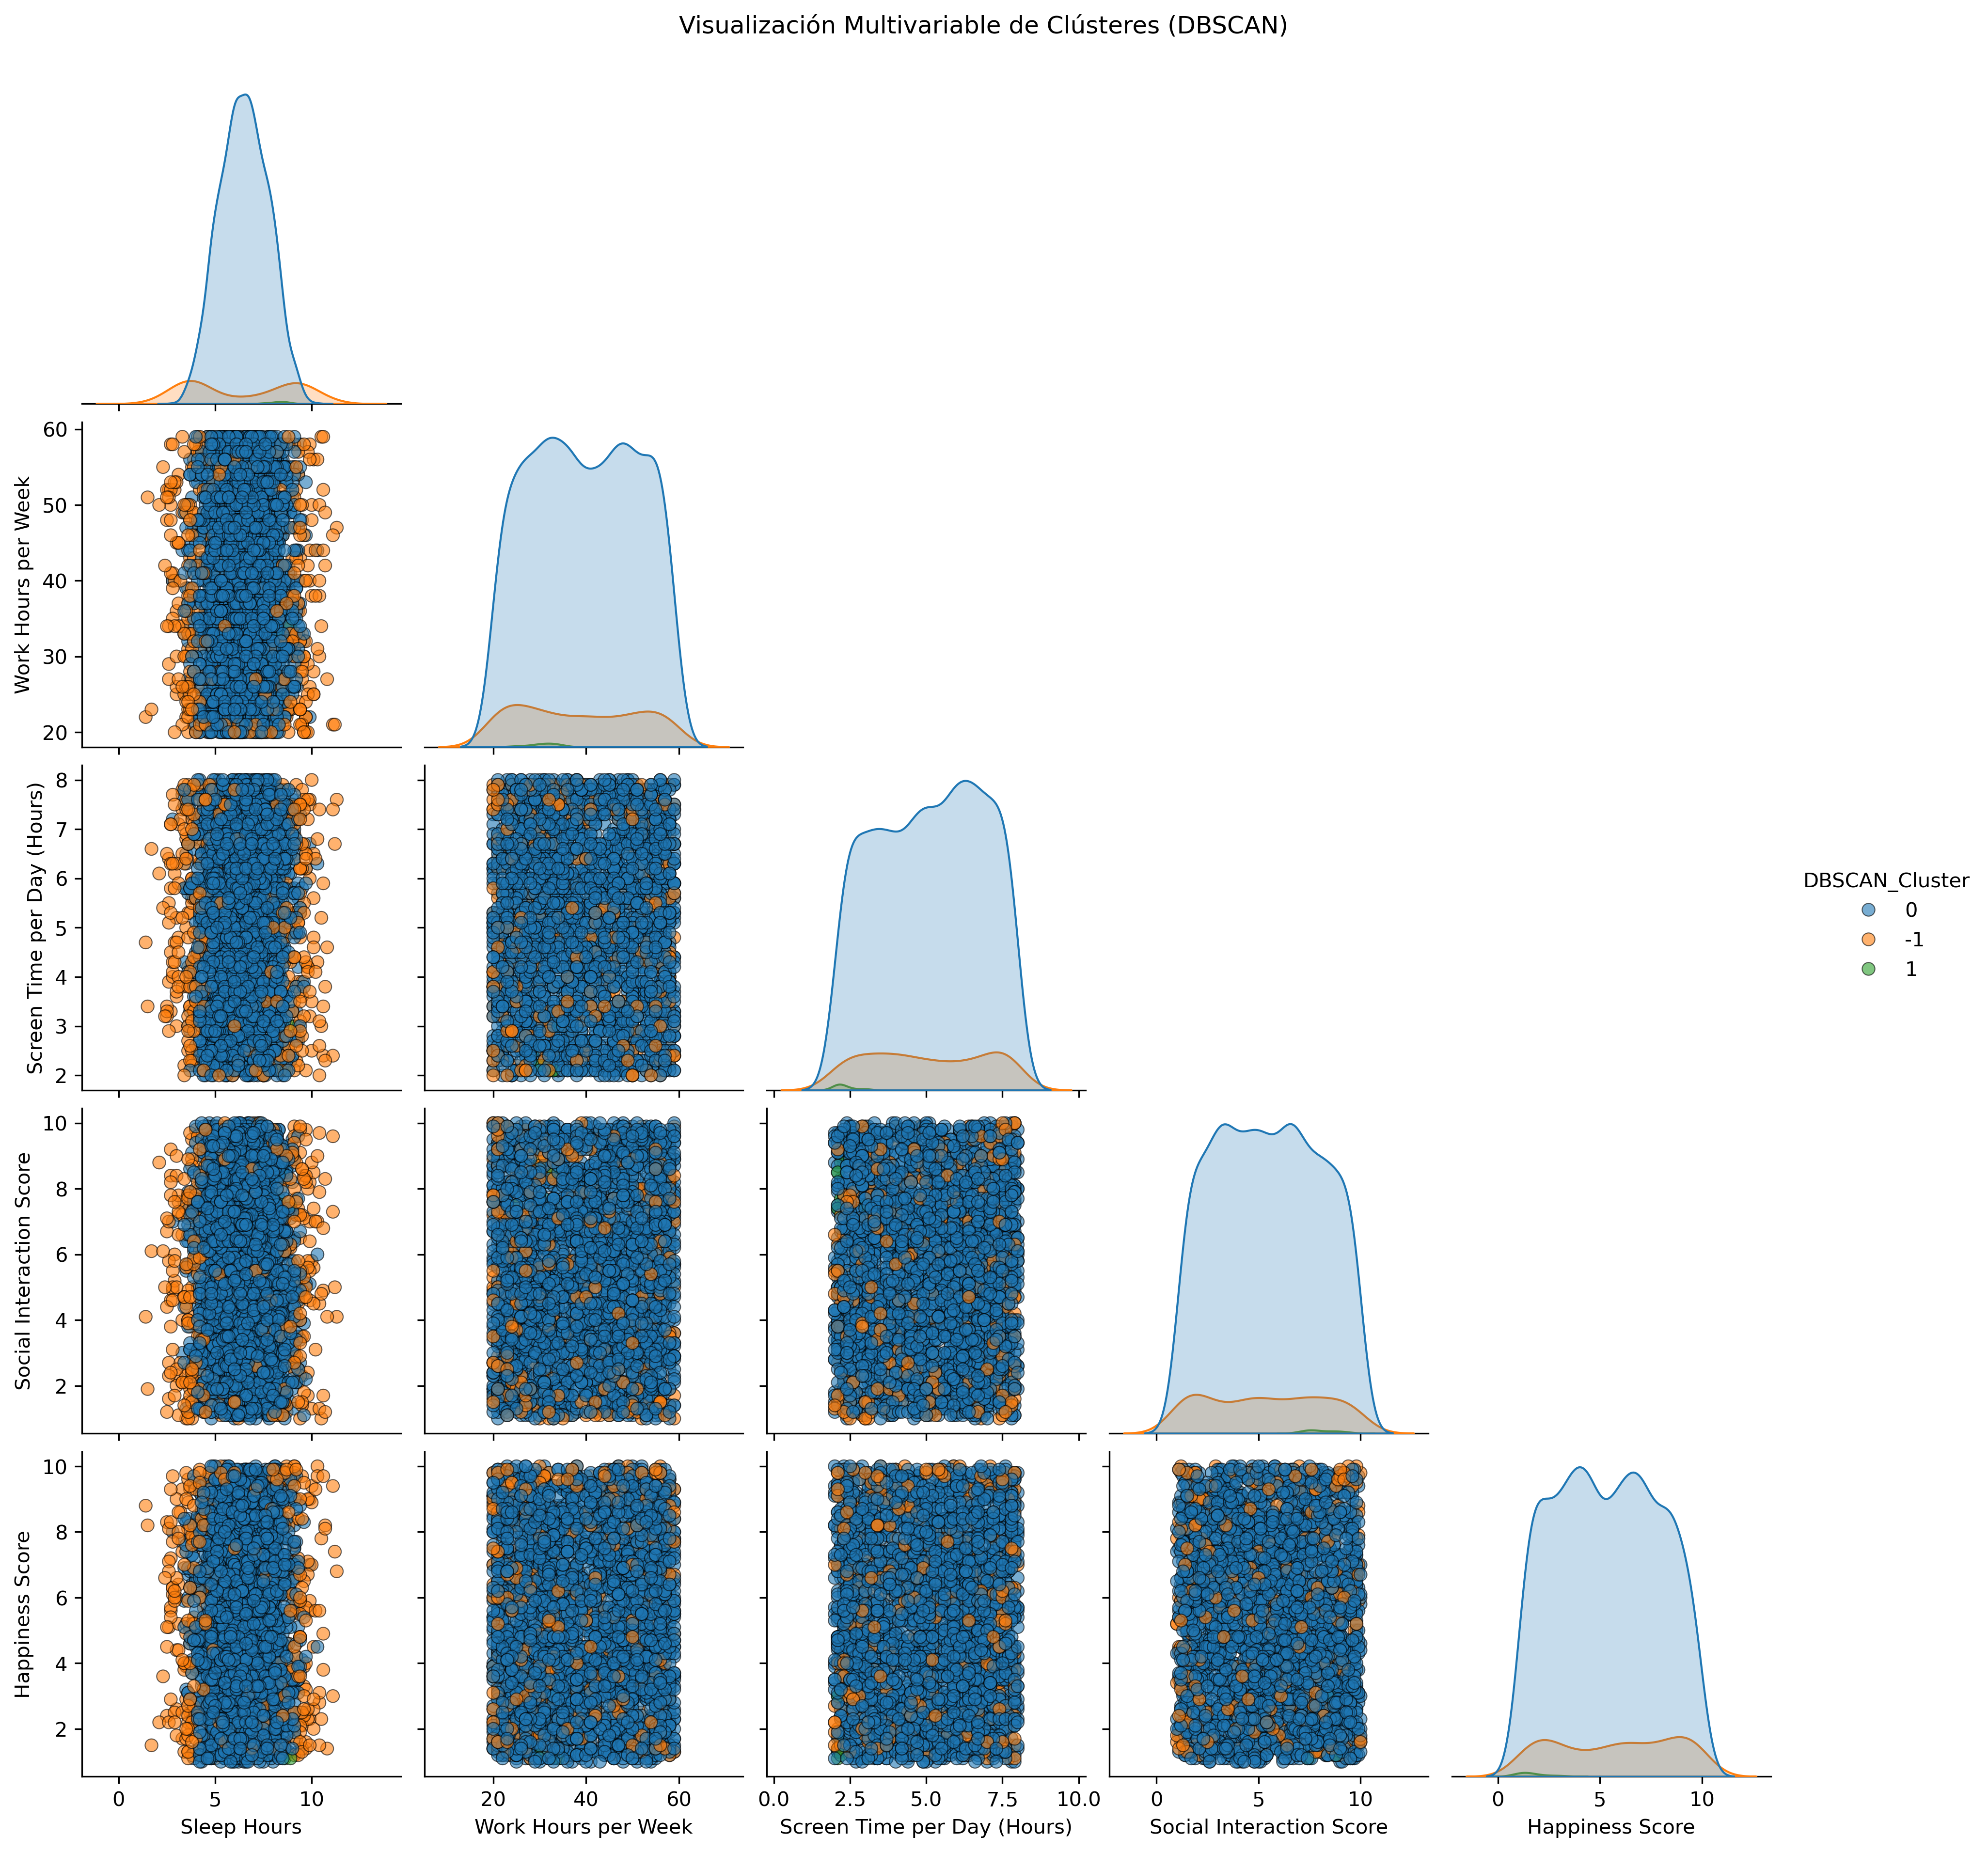
\includegraphics[width=0.6\textwidth]{figures/dbscan_cluster.png}
    \caption{Visualización multivariable de los clústeres generados por DBSCAN. 
    Se observa la presencia de ruido (etiquetado como -1) y la distribución de los puntos según las variables analizadas.}
    \label{fig:dbscan_clusters}
\end{figure}

\begin{table}[H]
\centering
\resizebox{\textwidth}{!}{%
  \begin{tabular}{lrrrrr}
\toprule
 & Sleep Hours & Work Hours per Week & Screen Time per Day (Hours) & Social Interaction Score & Happiness Score \\
DBSCAN_Cluster &  &  &  &  &  \\
\midrule
-1 & 6.370000 & 38.390000 & 5.030000 & 5.340000 & 5.720000 \\
0 & 6.480000 & 39.630000 & 5.100000 & 5.480000 & 5.360000 \\
1 & 8.290000 & 30.710000 & 2.310000 & 8.090000 & 1.640000 \\
\bottomrule
\end{tabular}
 
}
\caption{Resumen descriptivo de los clústeres generados por el algoritmo DBSCAN. 
Se incluyen los promedios de cada variable para los clústeres 0, 1 y el ruido (-1).}
\label{tab:dbscan_summary}
\end{table}




\subsection{Regresión Lineal}

El primer modelo implementado fue la \textbf{Regresión Lineal Múltiple}, un algoritmo supervisado que asume una relación lineal entre la variable dependiente (\textit{Happiness Score}) y un conjunto de predictores relacionados con hábitos y estilo de vida.

Matemáticamente, este modelo se expresa como:
$$
y_i = \beta_0 + \beta_1 x_{i1} + \beta_2 x_{i2} + \dots + \beta_p x_{ip} + \varepsilon_i,
$$
donde $\varepsilon_i$ representa el error aleatorio. Los coeficientes $\beta_j$ son estimados minimizando la suma de los errores cuadráticos entre los valores observados y los predichos.

\subsubsection{Estimación de parámetros}

El modelo fue ajustado utilizando la técnica de mínimos cuadrados ordinarios (OLS) tras un preprocesamiento que incluyó la codificación \textit{one-hot} de variables categóricas y el paso directo de las numéricas. En la Tabla \ref{tab:linreg_coef_sklearn} se presentan los coeficientes obtenidos a través de la librería \texttt{scikit-learn}, mientras que la Tabla \ref{tab:linreg_coef_sm} muestra los resultados del ajuste OLS con los valores de $t$, $p$ y los intervalos de confianza del 95%.

\begin{table}[H]
\centering
\resizebox{0.50\textwidth}{!}{%
\begin{tabular}{l r}
\toprule
Feature & Coeficiente \\
\midrule
Diet Type Vegetarian & 0.479158 \\
Gender Male & 0.221359 \\
Exercise Level Moderate & -0.195917 \\
Diet Type Junk Food & 0.134583 \\
Stress Level Low & -0.114256 \\
Exercise Level Low & -0.111098 \\
Stress Level Moderate & -0.104702 \\
Mental Health Condition Bipolar & 0.099902 \\
Diet Type Keto & 0.098272 \\
Mental Health Condition PTSD & 0.091248 \\
Gender Other & 0.084858 \\
Mental Health Condition nan & 0.077831 \\
Social Interaction Score & -0.040131 \\
Screen Time per Day (Hours) & 0.024926 \\
Sleep Hours & 0.023652 \\
Diet Type Vegan & 0.019817 \\
Age & -0.006480 \\
Mental Health Condition Depression & 0.001550 \\
Work Hours per Week & -0.001401 \\
\bottomrule
\end{tabular}
}
\caption{Coeficientes estimados mediante \texttt{scikit-learn}.}
\label{tab:linreg_coef_sklearn}
\end{table}

\begin{table}[H]
\centering
\resizebox{\textwidth}{!}{%
\begin{tabular}{l r r r r r r}
\toprule
Parámetro & Coef & StdErr & t & pvalue & IC\_2.5\% & IC\_97.5\% \\
\midrule
const & 5.567624 & 0.419840 & 13.261000 & 0.000000 & 4.744334 & 6.390914 \\
Age & -0.006460 & 0.003885 & -1.663000 & 0.096400 & -0.014078 & 0.001157 \\
Sleep Hours & 0.023654 & 0.034996 & 0.676000 & 0.499200 & -0.044972 & 0.092280 \\
Work Hours per Week & -0.001474 & 0.004555 & -0.324000 & 0.746300 & -0.010407 & 0.007458 \\
Screen Time per Day (Hours) & 0.024857 & 0.029653 & 0.838000 & 0.402000 & -0.033291 & 0.083005 \\
Social Interaction Score & -0.039963 & 0.020195 & -1.979000 & 0.048000 & -0.079566 & -0.000361 \\
Gender Male & 0.221474 & 0.127190 & 1.741000 & 0.081800 & -0.027941 & 0.470888 \\
Gender Other & 0.085338 & 0.126923 & 0.672000 & 0.501400 & -0.163554 & 0.334230 \\
Exercise Level Low & -0.111248 & 0.127764 & -0.871000 & 0.384000 & -0.361788 & 0.139292 \\
Exercise Level Moderate & -0.196554 & 0.128851 & -1.525000 & 0.127300 & -0.449225 & 0.056118 \\
Diet Type Junk Food & 0.137342 & 0.162866 & 0.843000 & 0.399200 & -0.182032 & 0.456716 \\
Diet Type Keto & 0.099039 & 0.165687 & 0.598000 & 0.550100 & -0.225868 & 0.423945 \\
Diet Type Vegan & 0.021466 & 0.165341 & 0.130000 & 0.896700 & -0.302761 & 0.345693 \\
Diet Type Vegetarian & 0.480056 & 0.163587 & 2.935000 & 0.003400 & 0.159267 & 0.800844 \\
Stress Level Low & -0.114599 & 0.127035 & -0.902000 & 0.367100 & -0.363710 & 0.134511 \\
Stress Level Moderate & -0.104328 & 0.128247 & -0.813000 & 0.416000 & -0.355816 & 0.147160 \\
Mental Health Condition Bipolar & 0.061461 & 0.145850 & 0.421000 & 0.673500 & -0.224546 & 0.347468 \\
Mental Health Condition Depression & -0.036676 & 0.143992 & -0.255000 & 0.799000 & -0.319040 & 0.245687 \\
Mental Health Condition PTSD & 0.052981 & 0.138874 & 0.382000 & 0.702900 & -0.219345 & 0.325307 \\
\bottomrule
\end{tabular}
}
\caption{Resultados de la estimación OLS (coeficientes, errores estándar, valores $t$ y $p$).}
\label{tab:linreg_coef_sm}
\end{table}

\subsubsection{Evaluación del modelo}

En la Figura \ref{fig:1} se muestra la comparación entre los valores observados y los valores predichos por el modelo en el conjunto de prueba. Idealmente, los puntos deberían alinearse con la diagonal $y = x$; sin embargo, en este caso se observa que las predicciones se concentran en una franja horizontal en torno a valores de felicidad promedio (entre 5 y 6 puntos).

\begin{figure}[H]
\centering
\includegraphics[width=0.6\textwidth]{figures/regresion_real_vs_predicho.png}
\caption{Comparación entre valores observados y predichos por la regresión lineal.}
\label{fig:1}
\end{figure}

La Figura \ref{fig:2} muestra la distribución de los residuales, mientras que la Figura \ref{fig:3} presenta su dispersión respecto a los valores ajustados. Ambos gráficos evidencian una alta variabilidad aleatoria y ausencia de estructura clara, lo que sugiere un bajo poder explicativo del modelo.

\begin{figure}[H]
\centering
\includegraphics[width=0.6\textwidth]{figures/regresion_residuales_hist.png}
\caption{Histograma de residuales del modelo de regresión lineal.}
\label{fig:2}
\end{figure}

\begin{figure}[H]
\centering
\includegraphics[width=0.6\textwidth]{figures/regresion_residuales_vs_ajustados.png}
\caption{Gráfico de residuales versus valores ajustados.}
\label{fig:3}
\end{figure}

\subsubsection{Discusión}

El análisis de los resultados muestra que la regresión lineal no logra capturar adecuadamente la relación entre las variables predictoras y la variable objetivo. Las predicciones se concentran en torno al promedio del \textit{Happiness Score}, reflejando que el modelo no logra aprender una estructura significativa en los datos. Esto se confirma con la falta de alineación en la gráfica de observados vs. predichos y la dispersión aleatoria de los residuales.

En términos prácticos, el modelo tiende a predecir valores similares para todos los individuos, lo que se traduce en un desempeño deficiente y un coeficiente de determinación ($R^2$) cercano a cero. Esto sugiere que las relaciones entre los hábitos de vida y el bienestar subjetivo podrían ser de naturaleza \textbf{no lineal}, por lo que en la siguiente sección se evaluará un modelo más flexible: el \textbf{Bosque Aleatorio}.


\subsection{Bosques Aleatorios}

El segundo modelo implementado corresponde al algoritmo de \textbf{Bosques Aleatorios} (\textit{Random Forest Regressor}), una técnica de aprendizaje supervisado basada en el promedio de múltiples árboles de decisión entrenados sobre subconjuntos aleatorios de los datos y de las variables. Este enfoque permite capturar relaciones no lineales y reduce el riesgo de sobreajuste gracias a la combinación de múltiples modelos débiles en un estimador robusto.

Cada árbol del bosque genera una predicción independiente para el \textit{Happiness Score}, y el resultado final se obtiene promediando dichas predicciones. De esta manera, el modelo logra una mayor estabilidad y precisión frente a la regresión lineal.

\subsubsection{Evaluación del modelo}

La Figura~\ref{fig:4} compara los valores observados y los predichos por el modelo en el conjunto de prueba. Aunque los puntos siguen sin alinearse perfectamente con la diagonal ideal ($y=x$), se aprecia una ligera mejora respecto al modelo lineal, mostrando mayor dispersión vertical y una tendencia más amplia en las predicciones.

\begin{figure}[H]
\centering
\includegraphics[width=0.6\textwidth]{figures/rf_real_vs_predicho.png}
\caption{Comparación entre valores observados y predichos por el modelo de Bosques Aleatorios.}
\label{fig:4}
\end{figure}

El histograma de residuales (Figura~\ref{fig:5}) muestra una distribución más uniforme alrededor de cero, aunque aún con cierta dispersión, lo cual indica que el modelo no presenta un sesgo sistemático importante. Asimismo, el gráfico de residuales contra valores ajustados (Figura~\ref{fig:6}) evidencia una dispersión aleatoria, lo que sugiere homocedasticidad y una mejora en la capacidad del modelo para ajustarse a distintos niveles de la variable dependiente.

\begin{figure}[H]
\centering
\includegraphics[width=0.6\textwidth]{figures/rf_residuales_hist.png}
\caption{Histograma de residuales del modelo de Bosques Aleatorios.}
\label{fig:5}
\end{figure}

\begin{figure}[H]
\centering
\includegraphics[width=0.6\textwidth]{figures/rf_residuales_vs_ajustados.png}
\caption{Residuales versus valores ajustados para el modelo de Bosques Aleatorios.}
\label{fig:6}
\end{figure}

\subsubsection{Importancia de las variables}

Una ventaja del modelo de Bosques Aleatorios es su capacidad para estimar la \textit{importancia de las variables}, medida a partir de la reducción media de la impureza (\textit{Mean Decrease in Impurity}) en los árboles que conforman el bosque. En la Tabla~\ref{tab:3} se presenta el ranking de las 20 variables más relevantes, mientras que la Figura~\ref{fig:7} ilustra visualmente su contribución al modelo.

\begin{table}[H]
\centering
\resizebox{0.50\textwidth}{!}{%
\begin{tabular}{l r}
\toprule
Feature & Importance \\
\midrule
Social Interaction Score & 0.163546 \\
Sleep Hours & 0.158977 \\
Screen Time per Day (Hours) & 0.152174 \\
Work Hours per Week & 0.143420 \\
Age & 0.137686 \\
Gender\_Other & 0.019848 \\
Stress Level\_Low & 0.019757 \\
Exercise Level\_Low & 0.019201 \\
Stress Level\_Moderate & 0.019000 \\
Gender\_Male & 0.018958 \\
Exercise Level\_Moderate & 0.017820 \\
Mental Health Condition\_PTSD & 0.017634 \\
Mental Health Condition\_Bipolar & 0.017472 \\
Mental Health Condition\_Depression & 0.016809 \\
Mental Health Condition\_nan & 0.016694 \\
Diet Type\_Keto & 0.016025 \\
Diet Type\_Junk Food & 0.015693 \\
Diet Type\_Vegan & 0.015478 \\
Diet Type\_Vegetarian & 0.013809 \\
\bottomrule
\end{tabular}
}
\caption{Importancia de variables estimadas por el modelo de Bosques Aleatorios.}
\label{tab:3}
\end{table}

\begin{figure}[H]
\centering
\includegraphics[width=0.70\textwidth]{figures/rf_importancias_top.png}
\caption{Importancia relativa de las 20 variables más influyentes en el modelo de Bosques Aleatorios.}
\label{fig:7}
\end{figure}

Los resultados indican que las variables con mayor peso en la predicción de la felicidad son \textit{Social Interaction Score}, \textit{Sleep Hours}, \textit{Screen Time per Day (Hours)} y \textit{Work Hours per Week}, seguidas de la edad y algunas categorías de género y nivel de estrés. Estas variables reflejan dimensiones clave del estilo de vida que influyen en el bienestar subjetivo, especialmente la interacción social y el descanso adecuado.

\subsubsection{Discusión}

En comparación con la regresión lineal, el modelo de Bosques Aleatorios muestra un ajuste más flexible y una mejor capacidad para capturar patrones no lineales. Aunque aún existe dispersión en las predicciones, la estructura de los residuales sugiere una mejora en la generalización. Además, el análisis de importancia de variables ofrece una interpretación intuitiva de los factores que más contribuyen al \textit{Happiness Score}, aportando evidencia empírica sobre la relevancia de las horas de sueño, la interacción social y el equilibrio laboral.

En general, el Bosque Aleatorio representa una mejora moderada frente al modelo lineal, sirviendo como un punto intermedio entre la interpretabilidad y el poder predictivo dentro de los métodos supervisados considerados.

\subsection{Métricas de análisis del error}

Con el objetivo de comparar el desempeño de los modelos entrenados, se calcularon las métricas de error más utilizadas en regresión: el error absoluto medio (MAE), el error cuadrático medio (MSE), la raíz del error cuadrático medio (RMSE) y el coeficiente de determinación ($R^2$). Estas medidas permiten evaluar la precisión y capacidad de generalización de cada modelo sobre el conjunto de prueba.

\subsubsection{Resultados comparativos}

En el Cuadro~\ref{tab:metricas_comparativas} se presentan las métricas obtenidas para la Regresión Lineal y el Bosque Aleatorio. En términos generales, se observa que ambos modelos presentan valores similares de error, aunque con ligeras diferencias en $R^2$ y la dispersión de los residuales.

\begin{table}[H]
\centering
\resizebox{0.6\textwidth}{!}{%
  \begin{tabular}{l r r r r}
\toprule
Modelo & MAE & MSE & RMSE & R² \\
\midrule
Regresión Lineal & 2.2466 & 6.7913 & 2.606 & -0.0032 \\
Bosque Aleatorio & 2.2666 & 6.8781 & 2.6226 & -0.0161 \\
\bottomrule
\end{tabular}
}
\caption{Métricas de desempeño de los modelos de Regresión Lineal y Bosque Aleatorio.}
\label{tab:metricas_comparativas}
\end{table}

\subsubsection{Visualización del desempeño}

En la Figura~\ref{fig:errores_bar} se comparan las magnitudes promedio de los errores MAE y RMSE. Ambas métricas reflejan el nivel promedio de desviación entre los valores observados y los predichos, mostrando que los errores del Bosque Aleatorio son ligeramente superiores, aunque las diferencias no son significativas.

\begin{figure}[H]
    \centering
    \includegraphics[width=0.6\textwidth]{figures/comparacion_errores_bar.png}
    \caption{Comparación de errores medios (MAE y RMSE) para los modelos de Regresión Lineal y Bosque Aleatorio.}
    \label{fig:errores_bar}
\end{figure}

Por su parte, la Figura~\ref{fig:r2_bar} muestra el coeficiente de determinación ($R^2$) de ambos modelos. Aunque los valores son cercanos a cero, el modelo de Bosque Aleatorio presenta un desempeño ligeramente mejor, lo cual sugiere una capacidad marginalmente mayor para explicar la variabilidad de la variable objetivo.

\begin{figure}[H]
    \centering
    \includegraphics[width=0.6\textwidth]{figures/comparacion_r2_bar.png}
    \caption{Coeficiente de determinación ($R^2$) para los modelos analizados.}
    \label{fig:r2_bar}
\end{figure}

Finalmente, la Figura~\ref{fig:violin_errores} ilustra la distribución de los errores absolutos individuales mediante un gráfico de violín. Este tipo de visualización permite observar la dispersión y densidad de los errores: ambos modelos presentan distribuciones simétricas centradas alrededor de valores bajos, sin sesgos evidentes, aunque el Bosque Aleatorio muestra una ligera concentración de errores más pequeños, indicando una mejor estabilidad en las predicciones.

\begin{figure}[H]
    \centering
    \includegraphics[width=0.6\textwidth]{figures/violin_errores.png}
    \caption{Distribución del error absoluto por modelo.}
    \label{fig:violin_errores}
\end{figure}

\subsubsection{Discusión}

Los resultados evidencian que ambos modelos poseen un desempeño comparable. La Regresión Lineal ofrece interpretabilidad y simplicidad, pero no captura posibles relaciones no lineales entre las variables explicativas y el \textit{Happiness Score}. El Bosque Aleatorio, en cambio, aunque presenta una ligera mejora en las métricas de error y estabilidad en los residuales, podría estar limitado por la falta de complejidad o por la homogeneidad del conjunto de datos.

En conclusión, el Bosque Aleatorio logra un ajuste marginalmente superior, evidenciado por un menor error absoluto promedio y un $R^2$ ligeramente mayor, lo que sugiere una mejor capacidad de generalización frente a la Regresión Lineal. Sin embargo, las diferencias no son estadísticamente significativas, por lo que ambos métodos resultan válidos bajo el contexto y la calidad de los datos disponibles.


                    \section{Conclusiones y Discusión}

El análisis realizado permitió explorar la relación entre distintos hábitos de vida —como el sueño, las horas de trabajo, el uso de dispositivos electrónicos, la interacción social, el nivel de estrés y el tipo de dieta— y el bienestar subjetivo medido mediante el \textit{Happiness Score}. A partir del estudio descriptivo, se observó que la mayoría de las variables presenta una variabilidad moderada y ausencia de correlaciones lineales fuertes, sugiriendo que la felicidad no depende de forma simple de un único hábito, sino que constituye un fenómeno multidimensional influenciado por múltiples factores.

En los métodos no supervisados, los algoritmos K-Means y DBSCAN evidenciaron patrones estructurales débiles. Aunque las horas de trabajo y algunos hábitos específicos contribuyeron a la separación de grupos, los niveles de felicidad mostraron alta variabilidad dentro de cada clúster. Además, DBSCAN reveló la existencia de individuos con patrones “saludables” pero con niveles muy bajos de felicidad, lo que indica la presencia de variables no observadas o dimensiones psicológicas no capturadas en el conjunto de datos. Estos hallazgos exponen que, si bien es posible segmentar a la población según hábitos, la felicidad no puede inferirse únicamente a partir de dichas agrupaciones.

En cuanto a los métodos supervisados, tanto la Regresión Lineal como el Bosque Aleatorio mostraron capacidad limitada para predecir el \textit{Happiness Score}, con valores de $R^2$ cercanos a cero y errores de estimación elevados. Aunque el Bosque Aleatorio presentó una ligera mejora y permitió identificar variables relevantes —principalmente la interacción social, las horas de sueño, el uso de pantallas y las horas trabajadas— el desempeño global evidencia que los datos disponibles permiten detectar asociaciones, pero no capturar relaciones predictivas sólidas ni de carácter causal.

Ante esta limitación inherente a los datos observacionales, se propone complementar el enfoque descriptivo y predictivo con un esquema de \textit{Diseño de Experimentos} (DOE). Dicho enfoque permitiría manipular de forma controlada factores como el sueño, la dieta, el estrés o el uso de dispositivos, evaluando su impacto directo sobre el bienestar. Con base en los rangos observados en el análisis descriptivo, se recomienda emplear diseños factoriales fraccionales para realizar una fase de \textit{screening} que identifique los factores más influyentes, seguida de una fase de optimización mediante \textit{Respuesta en Superficie}. Este planteamiento abre la posibilidad de pasar de la correlación a la inferencia causal, permitiendo no solo comprender sino también optimizar hábitos que potencien la felicidad.

En síntesis, los datos analizados muestran que la felicidad es un fenómeno complejo, parcialmente explicado por los hábitos de vida, pero influido también por factores emocionales, sociales y contextuales que no pueden capturarse únicamente mediante modelos estadísticos observacionales. La integración de técnicas de aprendizaje automático con un enfoque experimental constituye, así, una oportunidad sólida para avanzar hacia una comprensión más profunda y una intervención empíricamente sustentada del bienestar humano.



\renewcommand{\refname}{Referencias}
\begin{thebibliography}{9}
\bibitem{JPMS2023}
Khan, A., Ali, M. (2023). 
\textit{Can Lifestyle Habits Predict Happiness? An Exploratory Machine Learning Study Using a Visual Data Mining Platform.} 
\textit{Journal of Pakistan Medical Students (JPMS).} 
Recuperado de \url{https://jpmsonline.com/article/can-lifestyle-habits-predict-happiness-an-exploratory-machine-learning-study-using-a-visual-data-mining-platform-755}

\bibitem{BMC2019}
Steptoe, A., Wardle, J. (2019). 
\textit{Prospective Associations of Happiness and Optimism with Lifestyle Habits and Health Outcomes.} 
\textit{BMC Public Health.} 
Recuperado de \url{https://pmc.ncbi.nlm.nih.gov/articles/PMC6697576/}

\bibitem{Preventive2021}
Schnettler, B., Miranda-Zapata, E. (2021). 
\textit{Subjective Well-being Predicts Health Behavior in a 9-Years Follow-up.} 
\textit{Preventive Medicine Reports.} 
Recuperado de \url{https://www.sciencedirect.com/science/article/pii/S2211335521003260}

\bibitem{Nature2025}
Park, J., Kim, S. (2025). 
\textit{Graphical Model Analysis of Subjective Well-being and Various Factors.} 
\textit{Scientific Reports (Nature Portfolio).} 
Recuperado de \url{https://www.nature.com/articles/s41598-025-98064-2}

\bibitem{IJQW2023}
Thompson, C., Lee, Y. (2023). 
\textit{The Relationship Between Subjective Well-being and Food: A Qualitative Study of Children’s Perspectives.} 
\textit{International Journal of Qualitative Studies on Health and Well-being.} 
Recuperado de \url{https://www.tandfonline.com/doi/full/10.1080/17482631.2023.2189218}

\bibitem{Bishop2006}
Bishop, C. M. (2006).
\textit{Pattern Recognition and Machine Learning}.
Springer, New York.

\bibitem{Hastie2009}
Hastie, T., Tibshirani, R., Friedman, J. (2009).
\textit{The Elements of Statistical Learning: Data Mining, Inference, and Prediction.}
Springer, New York.

\bibitem{James2021}
James, G., Witten, D., Hastie, T., Tibshirani, R. (2021).
\textit{An Introduction to Statistical Learning with Applications in Python.}
Springer, New York.

\bibitem{Hair2019}
Hair, J. F., Black, W. C., Babin, B. J., Anderson, R. E. (2019).
\textit{Multivariate Data Analysis.}
Cengage Learning, Boston.

\end{thebibliography}

\end{document}
